%use lualatex/xelatex to compile this
\documentclass{scrartcl}
\usepackage{polyglossia}
\setdefaultlanguage{english}

\usepackage{marvosym}% für den Smiley :-)
\def\contradiction{\quad\text{\Large\Lightning}}
\usepackage{graphicx}
\usepackage{float}
\usepackage{listings}
\usepackage{color}
\usepackage{enumerate}

\lstset{%
  literate={ö}{{\"o}}1%
           {ä}{{\"a}}1%
           {ü}{{\"u}}1%
           {Ö}{{\"O}}1%
           {Ä}{{\"A}}1%
           {Ü}{{\"U}}1%
           {ß}{{\ss}}1%
}

\definecolor{bggray}{rgb}{0.90,0.90,0.90}
\definecolor{dkgreen}{rgb}{0.00,0.50,0.00}
\definecolor{mauve}{rgb}{0.50,0.00,0.30}
\definecolor{darkGray}{rgb}{0.40,0.40,0.40}
\lstset{%
  language=C++,                   % the language of the code
  basicstyle=\small\ttfamily,
  numbers=none,                   % where to put the line-numbers
  backgroundcolor=\color{bggray}, % choose the background color. You must add \usepackage{color}
  showspaces=false,               % show spaces adding particular underscores
  showstringspaces=false,         % underline spaces within strings
  showtabs=false,                 % show tabs within strings adding particular underscores
  frame=single,                   % adds a frame around the code
  tabsize=4,                      % sets default tabsize to 2 spaces
  breaklines=true,                % sets automatic line breaking
  breakatwhitespace=true,         % sets if automatic breaks should only happen at whitespace
  title=\lstname,                 % show the filename of files included with \lstinputlisting;
                                  % also try caption instead of title
  keywordstyle=\color{blue},      % keyword style
  commentstyle=\color{dkgreen},   % comment style
  stringstyle=\color{mauve},      % string literal style
  escapeinside={\%*}{*)},         % if you want to add a comment within your code
}

\usepackage{amsmath,amsfonts,amsthm,amssymb,bbm,dsfont,mathrsfs}
\delimitershortfall=-3pt %makes parentheses grow larger automagically

\DeclareMathOperator*{\argmin}{argmin}
\DeclareMathOperator{\argmax}{argmax}
\DeclareMathOperator*{\cupdot}{\stackrel{{}_\bullet}{\cup}}
\DeclareMathOperator*{\bigcupdot}{\stackrel{{}_\bullet}{\bigcup}}
\def\LHS{&\phantom{{}=}} % First line of align environment with no relation symbol should still be align with the other lines. This is a dirty fix.
\usepackage{txfonts}

%Komma und Punktabstände anpassen:
%\mathcode`,="013B %nervt, außerdem braucht niemand Kommazahlen.
%\mathcode`.="613A

\author{Stefan Walzer}

%MENGEN Symbole
\newcommand{\R}{\ensuremath{\mathbb R}}
\newcommand{\N}{\ensuremath{\mathbb N}}
\newcommand{\Z}{\ensuremath{\mathbb Z}}
\newcommand{\Q}{\ensuremath{\mathbb Q}}
\newcommand{\C}{\ensuremath{\mathbb C}}
\newcommand{\K}{\ensuremath{\mathbb K}}

%Quantoren
\newcommand{\E}{\ensuremath{\exists}}
\newcommand{\A}{\ensuremath{\forall}}

%Pfeile
\newcommand{\LA}{\ensuremath{\Leftarrow}}
\newcommand{\RA}{\ensuremath{\Rightarrow}}
\newcommand{\la}{\ensuremath{\leftarrow}}
\newcommand{\ra}{\ensuremath{\rightarrow}}
\newcommand{\LRA}{\ensuremath{\Leftrightarrow}}
\newcommand{\lra}{\ensuremath{\leftrightarrow}}
\newcommand{\LLRA}{\ensuremath{\Longleftrightarrow}}
\newcommand{\llra}{\ensuremath{\longleftrightarrow}}

%spitze Klammern
\newcommand{\lan}{\ensuremath{\langle}}
\newcommand{\ran}{\ensuremath{\rangle}}


%Symbole
\newcommand{\veps}{\ensuremath{\varepsilon}}

%Verknüpfungen
\newcommand{\AND}{\wedge} %und
\newcommand{\OR}{\vee} %oder
\newcommand{\UN}{\cup} %union
\newcommand{\IS}{\cap} %intersection

%sonstiges
\def\abs#1{\left|#1\right|}
\def\norm#1{\lVert#1\rVert}
\def\floor#1{\left\lfloor#1\right\rfloor}
\def\ceil#1{\left\lceil#1\right\rceil}
\def\enquote#1{\glqq #1 \grqq}

\def\powset#1{\mathscr{P}\left(#1\right)}
\def\set#1{\left\{#1\right\}}
\def\setgen#1#2{\left\{#1\;\middle|\;#2\right\}}

%vector
\newcommand{\vect}[1]{\begin{pmatrix}#1\end{pmatrix}}
\newcommand{\svect}[1]{\scalebox{0.7}{$\begin{pmatrix}#1\end{pmatrix}$}}

%Fonts:

\setmainfont[Ligatures=TeX,SmallCapsFont={Latin Modern Roman Caps}]{Georgia}
\setsansfont{Segoe UI}
\setmonofont{Consolas}
\usepackage{unicode-math}
\setmathfont{xits-math.otf}

\usepackage{newunicodechar}
\newunicodechar{Ø}{\emptyset}

\begin{document}
    \section*{Exercise 7}
    
    Let $P_1$ and $P_2$ be projectives, $e : E → X$ any epimorphism and $f : P_1 + P_2 → X$. We need to show that $f$ factorises through $e$.
    
    We start with the solid lines in the following diagram.
    \begin{figure}[h]
        \centering
        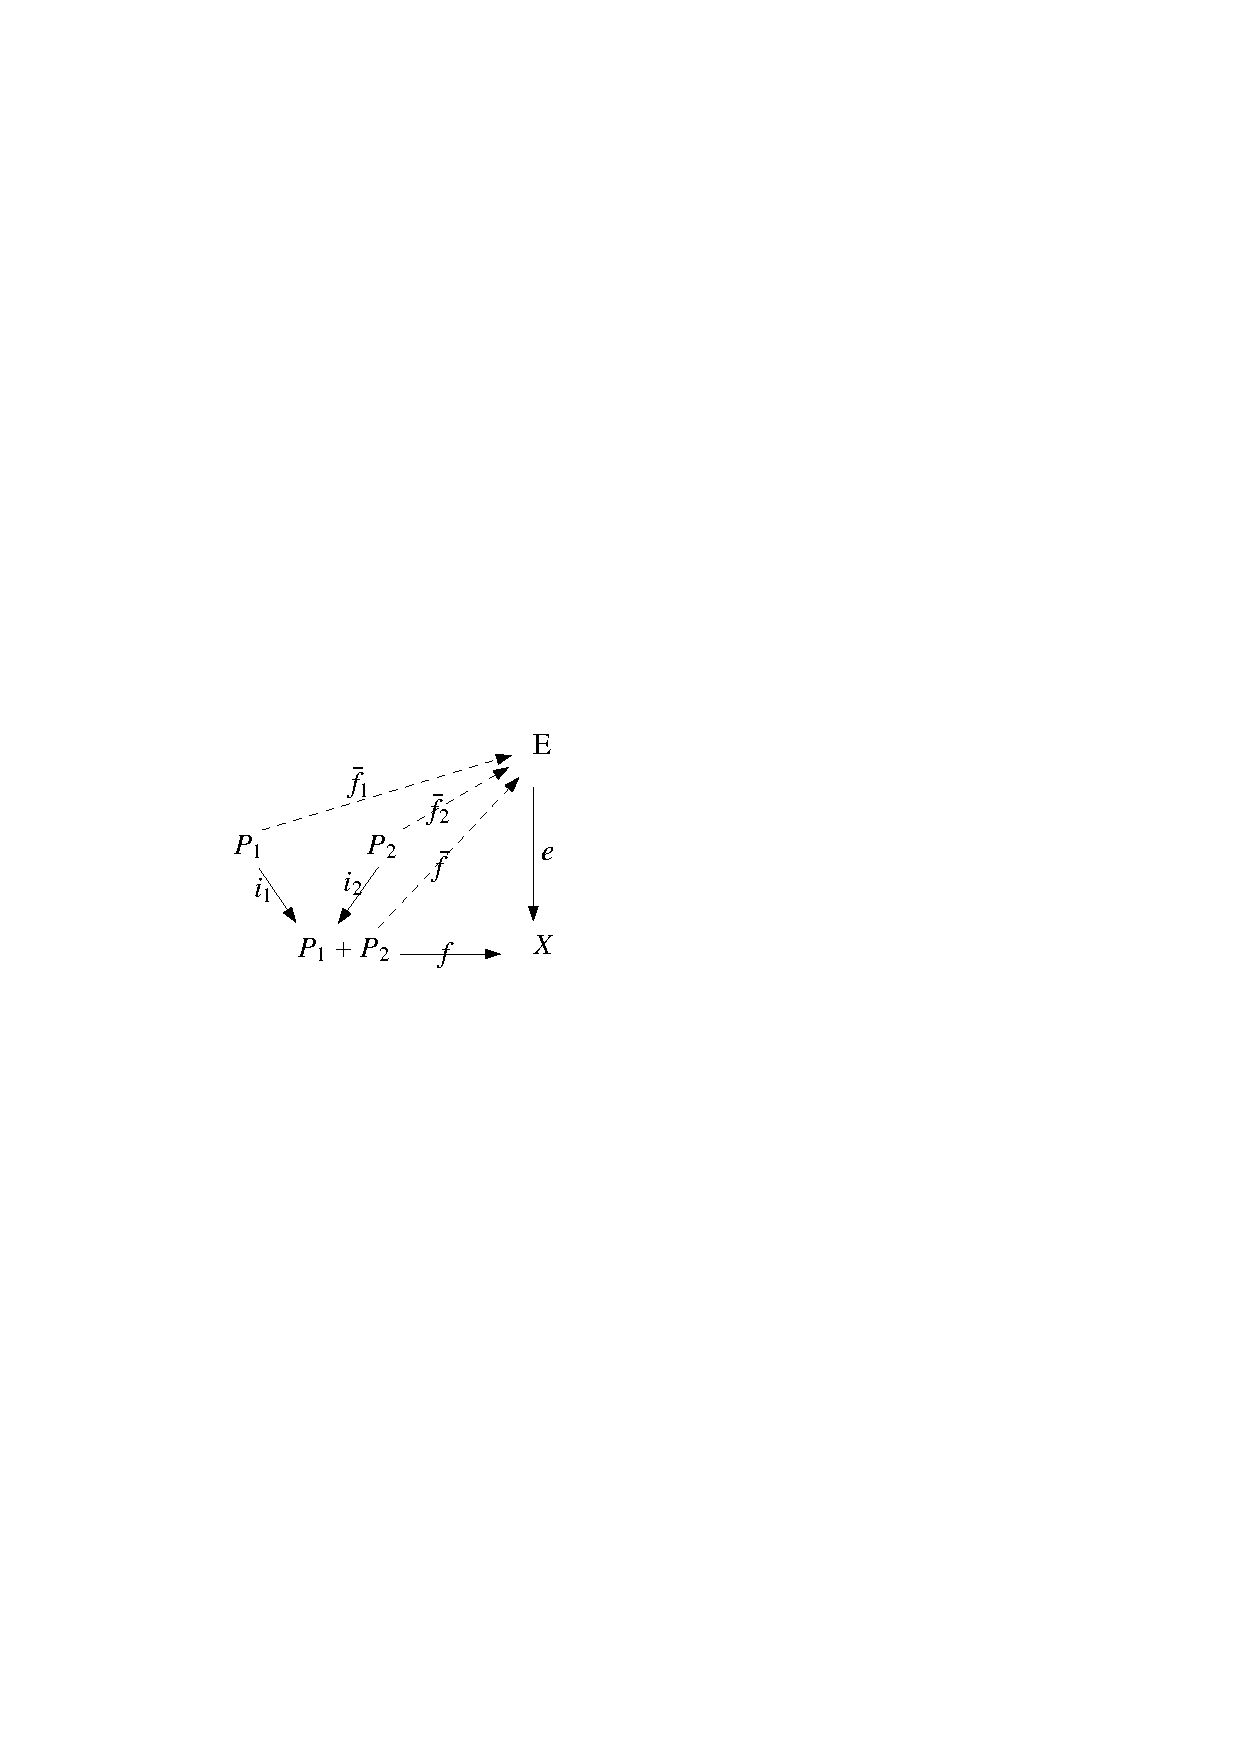
\includegraphics[width=0.5\textwidth]{stefan_fig.pdf}
    \end{figure}
    
    Because $P_1$ is a projection, the function $f \circ i_1$ factorises over $E$ (call the function $\bar{f}_1$). The same holds for $P_2$. Now we can use the universal property of the coproduct and construct $\bar{f}$ such that $\bar{f} \circ i_1 = \bar{f_1}$ and $\bar{f} \circ i_2 = \bar{f_2}$
    
    Now all paths starting from $P_1$ and $P_2$ commute. Using the universal property of the coproduct again, we see that $e \circ \bar{f}$ and $f$ both go from $P_1 + P_2$ to $X$ and must therefore be the same (unique) morphism that makes the diagram comute and we are done since we have found $e \circ \bar{f} = f$.
    
    \section*{Exercise 15}
    
    Let $f, g: X → Y$ be two morphisms in {\bf Top}. I claim the coequaliser of $f$ and $g$ is the projection $π$ to $Y/{\sim}$ where $\sim$ is the smallest equivalence relation containing $\setgen{(f(x), g(x))}{x ∈ X}$.
    
    This means, that $Y/{\sim}$ is the space of equivalence classes of $\sim$ and the open sets are exactly those sets $S$ such that $π^{-1}(S)$ is open in $Y$, where $π$ denotes the projection $x \mapsto [x]_{\sim}$. It is simple to check that this indeed constitutes a valid topology.
    
    Now for the universal property: Assume there is a morphism $c : Y → Z$ such that $c \circ f = c \circ g$. This means that $c$ respects $\sim$, namely $y_1 \sim y_2 ⇒ c(y_1) = c(y_2)$. Therefore $c^{*} : Y/{\sim} → Z$ given by $[x]_\sim \mapsto c(x)$ is a well-defined function such that $c^{*} \circ π = c$. It is also continuous since, if $O ⊂ Z$ is open, then so is $c^{*-1}(O) ⊂ Y$ because this just means that $π^{-1}(c^{*-1}(O)) = c^{-1}(O)$ must be open which is true because $c$ is continuous. It is obvious, that we could not have defined $c^{*}$ differently, so the factorisation over $Y/{\sim}$ is unique as we want it to be.
\end{document}